\documentclass{beamer}

\usepackage{beamerthemesplit}
\usepackage{amsmath}
\usepackage[fleqn]{mathtools}
\DeclareMathOperator*{\argmin}{arg\,min}

\usepackage{tikz}
\usetikzlibrary{positioning}

\addtobeamertemplate{background canvas}{\transfade}{}

\newcommand*{\vcenterimage}[2][]{\vcenter{\hbox{\includegraphics[#1]{#2}}}}
\newcommand*{\vcenterarrow}{\vcenter{\hbox{$\Longrightarrow$}}}

\title{Keyword Search Based on WFST Indexing}
\author{Wang Jian}
\date{Feb. 2, 2016}

\begin{document}

\setbeamercovered{transparent}

\frame{\titlepage}

\section[Outline]{}
\frame{\tableofcontents}

\section{Introduction}
\subsection{Keyword Search}
\frame
{
  \frametitle{\subsecname}
  
  \begin{itemize}
  \item{also known as Spoken Term Detection}

  \item{Traditional Approaches}
  
      \begin{itemize}
      \item{LVCSR-based} 
        \begin{itemize}
        \item{LVCSR followed by a text searching}
         \end{itemize}
         
      \item{Acoustic KWS} 
        \begin{itemize}
        \item{Viterbi search on a network consists of keywords and garbage models}
         \end{itemize}
      
      \item{Phonetic Search} 
        \begin{itemize}
        \item{search on a lattice of phonemes}
         \end{itemize}
            
      \end{itemize}

  \end{itemize}
}

\section{WFST-based Keyword Search}
\subsection{WFST-based Indexing}
\frame
{
  \frametitle{\subsecname}
  
  \begin{itemize}
  \item<1->{Indexation WFST($T$)}
    \begin{itemize}
    \item{every path of indexation WFST represents}
      \begin{itemize}
      \item{input: keyword}
      \item{output: all utterances contain the keyword (with timing information)}
      \end{itemize}
    \end{itemize}
 
  \item<2->{Search Method}
    \begin{itemize}
    \item{convert keyword to a WFST($T$)}
    \item{compose two WFSTs $R = X \circ T$}
    \item{paths on $R$ produce the result utterance set}
    \end{itemize}
  \end{itemize}
}

\frame
{
  \frametitle{\subsecname}
  
  \begin{itemize}
  \item{Factor WFST}
    \begin{itemize}
    \item{Given two strings $u$ and $v$, v is a \emph{factor} (substring) of $u$, if $u = xvy$ for some $x$ and $y$}
    \item{The \emph{factor WFST} $F(u)$ of a string $u$ is the minimal deterministic WFST recognizing exactly the set of factors of $u$}
    \end{itemize}
  \end{itemize}
  
  $\vcenterimage[width=.3\textwidth]{wfst.png}\vcenterarrow\vcenterimage[width=.3\textwidth]{factor.png}\vcenterarrow\vcenterimage[width=.3\textwidth]{opt_factor.png}$
}

\subsection{Utterance Level Keyword Search}
\frame
{
  \frametitle{\subsecname}
  
  \begin{itemize}
  \item<1->{Indexing}
    \begin{enumerate}
    \item{run a LVCSR system and output a lattice for every utterance}
    \item{convert every lattice to a WFST($A$) with word/phoneme as input/output and probability as weight}
    \item{construct $F(A)$ for every $A$}
    \item{take the union of all $F(A)$s}
    \end{enumerate}
    
  \item<2->{Searching}
    \begin{enumerate}
    \item{convert query/keyword to a WFST($X$)}
    \item{compose the two WFST $R = \Pi_2(X \circ T)$}
    \item{extract the most likely paths of $R$}
    \end{enumerate}
  \end{itemize}
}

\subsection{Timed Keyword Search}
\frame
{
  \frametitle{\subsecname}
  
  \begin{itemize}
  \item{Cluster the arcs with the same input label and overlapping time-spans.}
  \end{itemize}
  
   $\vcenterimage[width=.4\textwidth]{wfst.png}\vcenterarrow\vcenterimage[width=.5\textwidth]{wfst_cluster.png}$
}

\frame
{
  \frametitle{\subsecname}
  
  \begin{itemize}
  \item{generate factor with timing informations}
  \end{itemize}
  
   \centering{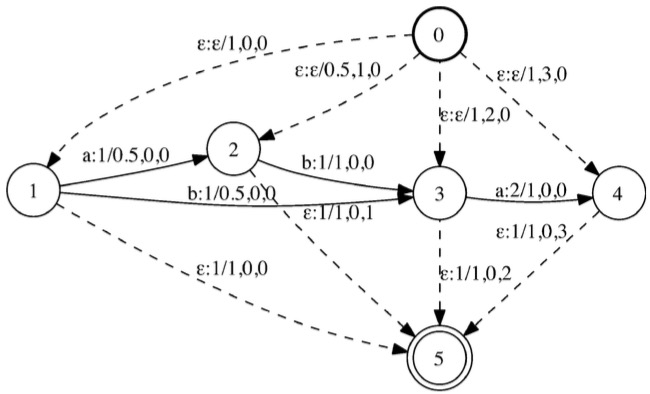
\includegraphics[width=.6\textwidth]{factor_timing.png}}
 }

\frame
{
  \frametitle{\subsecname}
  
  \begin{itemize}
  \item{merge arc with same input-output pair(overlapped labels)}
  \end{itemize}
  
   \centering{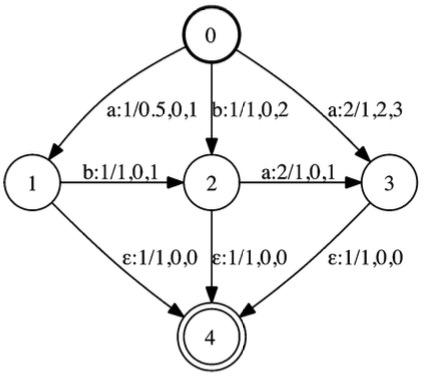
\includegraphics[width=.6\textwidth]{factor_merging.png}}
}

\frame
{
  \frametitle{\subsecname}
  
  \begin{itemize}
  \item{factor disambiguation}
  \end{itemize}
  
   \centering{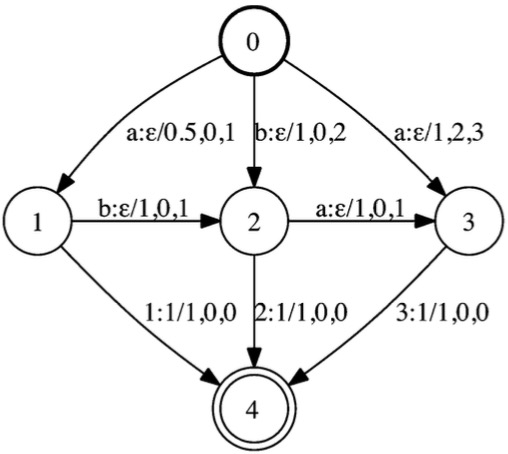
\includegraphics[width=.6\textwidth]{factor_disambiguation.png}}
}

\frame
{
  \frametitle{\subsecname}
  
  \begin{itemize}
  \item{factor optimization}
  \end{itemize}
  
   \centering{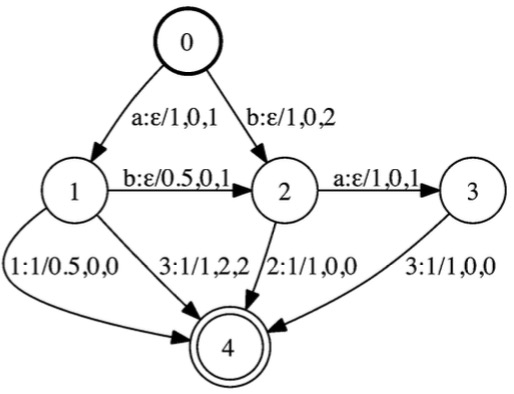
\includegraphics[width=.6\textwidth]{factor_timing_opt.png}}
}

\section{Experiments}
\subsection{Setup}
\frame
{
  \frametitle{\subsecname}
  
  \begin{itemize}
    \item \textbf{Scripts} Kaldi \texttt{egs/babel/s5c/}
    \item \textbf{dataset} 57904 utters, 41 hours
    \item \textbf{model} SAT fmllr gmm model (tri5a) with same dataset
  \end{itemize}
}

\subsection{Results}
\frame
{
  \frametitle{\subsecname}
  
        \begin{tabular}{l|r|r|r|r|r}
           lmwt              &   ATWV    &    OTWV   &  STWV   &  MTWV/THRESH  &  Recall \\
           \hline
           \hline
           8                     &    0.5750   &    0.6318   &   0.9618 &  0.6318/0.260               & 0.9627 \\
           9                     &    0.5767   &    0.6353   &   0.9618 &  0.6353/0.305               & 0.9627 \\
           10                   &    0.5818   &    0.6352   &   0.9618 &  0.6291/0.252               & 0.9627 \\
           11                   &    0.5750   &    0.6410   &   0.9618 &  0.6275/0.291               & 0.9627 \\
           12                   &    0.5803   &    0.6352   &   0.9618 &  0.6237/0.299               & 0.9627 \\
        \end{tabular}
}

\section{References}
\frame
{
  \frametitle{\secname}
  
   \begin{itemize}
     \item utterance level search
       \begin{itemize}
       \item Allauzen, Cyril, Mehryar Mohri, and Murat Saraclar. “General Indexation of Weighted Automata: Application to Spoken Utterance Retrieval.” In Proceedings of the Workshop on Interdisciplinary Approaches to Speech Indexing and Retrieval at HLT-NAACL 2004, 33–40.
       \end{itemize}

     \item timed search
       \begin{itemize}
       \item Can, Doğan, and Murat Saraclar. “Lattice Indexing for Spoken Term Detection.” Audio, Speech, and Language Processing, IEEE Transactions on 19, no. 8 (2011): 2338–47.
       \end{itemize}          
  \end{itemize}
}

\end{document}
